\chapter{Ramping parameter under the random graph model} % (fold)
\label{cha:ramping_parameter_under_the_random_graph_model}

The previous work~\cite{Sindel:2009vd} provided a connection between the clustered structure of a graph and an interpretation of concentration risk.
The methodology presented by the authors considered the effects of removing edges with weight under given a varying threshold on the community structure of a fully connected obligor-correlation matrix.

This thesis approaches a different problem.
In particular, it tries to describe the expected behaviour of the curve designed by the~\cite{Sindel:2009vd} the problem from the perspective of having
large, idealized portfolios 
and a random graph model that generates them.


In this chapter, we will be considering random graphs generated by the 

We will not be considering individual instances of graphs, but rather the population effects on them.



assumption:
weights are uniformly distributed and independent
exposure on nodes is independently distributed from the weights of the vertices


\begin{figure}[tb]
	\centering
	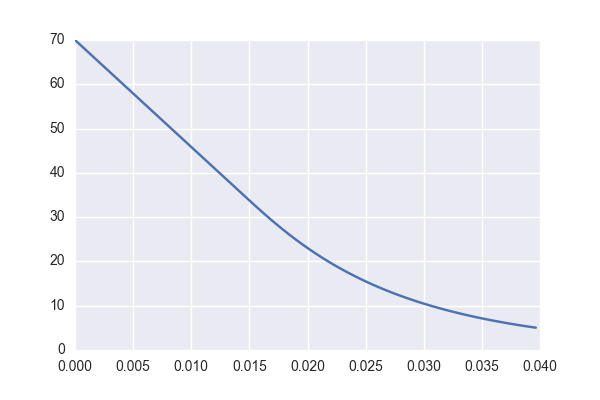
\includegraphics[]{figures/gnp_number_components.png}
	\caption{Number of components as a function of the probability $p$ of the $G(n,p)$ model.}
	\label{fig:figure1}
\end{figure}


\begin{itemize}
	\item The variation of the ramping parameter is equivalent to having random graphs generated with different $p$ probabilities
\end{itemize}


describe the phase transition


describe the size of the components


% chapter ramping_parameter_under_the_random_graph_model (end)